\documentclass{sig-alternate-05-2015}
%\documentclass{llncs}
\usepackage{makeidx}
\usepackage{tabularx,colortbl}
%\usepackage[dvipsnames]{xcolor}
\usepackage{flushend}
\usepackage{cite}
\usepackage{amsmath}
%\usepackage{amsthm}
\usepackage{amssymb}
\usepackage{epsfig}
\usepackage{stmaryrd}
\usepackage{url}
\usepackage{multirow}
\usepackage{latexsym}
\usepackage{graphics}
\usepackage{graphicx}
\usepackage{enumitem}
\usepackage{comment}
\usepackage{longtable}
\usepackage{supertabular}
\usepackage{times}
\usepackage{listings}
\usepackage{subfigure}
\usepackage{color}
\usepackage{balance}
\usepackage{xspace}
\usepackage[ruled, vlined, linesnumbered]{algorithm2e}
\usepackage[autostyle]{csquotes}
\usepackage{caption}



%\theoremstyle{Definition}
%\newtheorem{definition}{Definition}
%%%
%\theoremstyle{Theorem}
%\newtheorem{theorem}{Theorem}


%\newcommand{\definition}{\noindent \textbf{Definition} \citation{}}
%\newcommand{\theorem}{\noindent \textbf{Theorem} \citation{}}
%\newcommand{\lemma}{\noindent \textbf{Lemma} \citation{}}

%\newdef{lemma}{Lemma}
%\newdef{definition}{Definition}
%\newdef{theorem}{Theorem}
%\newdef{corollary}{Corollary}
%\newdef{note}{Note}
%\newdef{axiom}{Axiom}
\newcommand{\mkeyword}[1]{\mbox{\texttt{#1}}}
\DeclareMathOperator{\kuop}{uop}
\DeclareMathOperator{\kbop}{bop}
\DeclareMathOperator{\kite}{ite}
\DeclareMathOperator{\kpre}{pre}
\DeclareMathOperator{\dom}{dom}
\DeclareMathOperator{\ktrue}{true}
\DeclareMathOperator{\kfalse}{false}
\DeclareMathOperator{\kselect}{select}
\DeclareMathOperator{\ran}{range}
%\definecolor{mypink}{rgb}{0.858, 0.188, 0.478}
\newcommand{\lbb}{[\![}
\newcommand{\rbb}{]\!]}
\newcommand{\expr}{\phi}
\newcommand{\exprS}{\Phi}
%\newcommand{\mike}[1]{\textcolor{red}{#1}}
%\newcommand{\janet}[1]{\textcolor{blue}{#1}}
%\newcommand{\darren}[1]{\textcolor{green}{#1}}
%\newcommand{\danielle}[1]{\textcolor{orange}{#1}}

%\sloppypar
\usepackage{etoolbox}
\makeatletter
\patchcmd{\maketitle}{\@copyrightspace}{}{}{}
\makeatother


\begin{document}
%\CopyrightYear{2016}
%\setcopyright{acmcopyright}
%\conferenceinfo{FSE'16,}{November 13-19, 2016, Seattle, WA, USA}
%\isbn{978-1-4503-4218-6/16/11}\acmPrice{\$15.00}
%\doi{http://dx.doi.org/10.1145/2950290.2950346}

\definecolor{gold}{rgb}{0.90,.66,0}
\definecolor{dgreen}{rgb}{0,0.6,0}
\newcommand{\stateequiv}{\equiv_{s}}
\newcommand{\traceequiv}{\equiv_{\sigma}}
\newcommand{\ta}{\text{TA}}
\newcommand{\cta}{\text{TA$_{C}$}}
\newcommand{\tta}{\text{TA$_{T}$}}
\newcommand{\ucalg}{\texttt{\small{IVC\_UC}}}
\newcommand{\ucbfalg}{\texttt{\small{IVC\_UCBF}}}
\renewcommand{\abstract}{\noindent {\sc \textbf{\large {Abstract}}}\\}


% paper title
% can use linebreaks \\ within to get better formatting as desired
\title{Written Preliminary Examination Report: Architectural Modeling and Analysis for Safety Engineering}
%\subtitle{[subtitle]
%\titlenote{A full version of this paper is available as
%\textit{Author's Guide to Preparing ACM SIG Proceedings Using
%\LaTeX$2_\epsilon$\ and BibTeX} at
%\texttt{www.acm.org/eaddress.htm}}}
\numberofauthors{1} %  in this sample file, there are a *total*
% of EIGHT authors. SIX appear on the 'first-page' (for formatting
% reasons) and the remaining two appear in the \additionalauthors section.
%
\author{
% You can go ahead and credit any number of authors here,
% e.g. one 'row of three' or two rows (consisting of one row of three
% and a second row of one, two or three).
%
% The command \alignauthor (no curly braces needed) should
% precede each author name, affiliation/snail-mail address and
% e-mail address. Additionally, tag each line of
% affiliation/address with \affaddr, and tag the
% e-mail address with \email.
%
% 1st. author
\alignauthor
Danielle Stewart\\
       \affaddr{Department of Computer Science \& Engineering}\\
       \affaddr{University of Minnesota}\\
       \affaddr{MN, USA}\\
       \email{dkstewar@umn.edu}
       }



\maketitle

\begin{abstract}
This paper describes a new methodology with tool support for model-based safety analysis. The tool support is implemented as a {\em Safety Annex} for the Architecture Analysis and Design Language (AADL). The Safety Annex provides the ability to describe faults and faulty component behaviors in AADL models. In contrast to previous AADL-based approaches, the Safety Annex leverages a formal description of the nominal system behavior to propagate faults in the system. This approach ensures consistency with the rest of the system development process and simplifies the work of safety engineers. The language for describing faults is extensible and allows safety engineers to weave various types of faults into the nominal system model. The Safety Annex supports the injection of faults into component level outputs, and the resulting behavior of the system can be analyzed using model checking through the Assume-Guarantee Reasoning Environment (AGREE).
\end{abstract}

\keywords{Model-based systems engineering; fault analysis; safety engineering}

\section{Introduction}
\label{sec:intro}

Risk and safety analyses are important activities used to ensure that critical systems operate in an expected way. From nuclear power plants and airplanes to heart monitors and automobiles, critical systems are ubiquitous in our society. These systems are required to operate safely under nominal and faulty conditions. Guaranteeing that system safety properties hold in the presence of faults is an important aspect of critical systems development and falls under the discipline of safety analysis. Safety analysis produces various safety related artifacts that are used during development and certification of critical systems~\cite{SAE:ARP4761,SAE:ARP4754A}. Examples include {\em minimal cut sets} -- the minimal sets of faults that may violate a safety property and {\em fault trees} -- the Boolean formula whose literals are minimal cut sets. Since the introduction of minimal cut sets in the field of safety analysis~\cite{vesely1981fault}, much research has been performed to address the generation of these sets and associated formulae~\cite{fta:survey,rauzy1993new,historyFTA,Bozzano:2010:DSA:1951720,rausand2003system}. As critical systems get larger, more minimal cut sets are possible with increasing cardinality. In recent years, symbolic model checking has been used to address scaling the analysis of systems with millions of minimal cut sets~\cite{bieber2002combination,schafer2003combining,fta:survey,contractBasedDesign,symbFTA,DBLP:conf/cav/BozzanoCPJKPRT15}. 

The state space explosion problem often prevents formal verification from being used on large systems. This problem can arise from combining parallel processes together and attempting to reason monolithically over them. Compositional reasoning takes advantage of the hierarchical organizaton of a system model. A compositional approach verifies each component of the system in isolation and allows global properties to be inferred about the entire system~\cite{berezin1997compositional}. The {\em assume-guarantee} paradigm is commonly used in compositional reasoning where the assumed behavior of the environment implies the guaranteed behavior of the component ~\cite{NFM2012:CoGaMiWhLaLu}.

Using an assume-guarantee reasoning framework, we extend the definition of the nomimal transition system to allow for unconstrained guarantees. We use this idea to generate all counterexamples to a proof for each layer of analysis, and then transform the results into a Boolean formula describing the satisfiability of the violation of a property. These results are then composed. 

After we provide the formalization, we describe the implementation in the OSATE tool for the Architecture and Analysis Lanugage (AADL)~\cite{FeilerModelBasedEngineering2012}. AADL has two annexes that are of interest to us: the Assume-Guarantee Reasoning Environment (AGREE)~\cite{NFM2012:CoGaMiWhLaLu} and the safety annex~\cite{stewart2020safety}. AGREE provides the assume-guarantee reasoning required for the transition system extension and the safety annex allows us to define faults on component outputs. 

Recently, Ghassabani et al. developed an algorithm that traces a safety property to a minimal set of model elements necessary for proof; this is called the \textit{all minimal inductive validity core} algorithm (\aivcalg)~\cite{GhassabaniGW16,Ghassabani2017EfficientGO,bendik2018online}. Inductive validity cores produce the minimal set of model elements necessary to prove a property. Each set contains the \emph{behavioral contracts} -- the requirement specifications for components -- used in a proof. We collect all MIVCs per layer to generate the minimal cut sets and thus the fault trees to be composed.

%The \aivcalg algorithm gives the minimal set of contracts required for proof of a safety property. If all of these sets are obtained, we have insight into every proof path for the property. Thus, if we violate at least one contract from every MIVC set, we have in essence ``broken" every proof path. This is the information that is used to perform fault analysis using MIVCs.

%If all of these sets are obtained, we have insight into not only what is necessary for the verification of the property, but we can also find what combination of contracts, if \emph{violated}, will provide a state of the system which makes the safety property unprovable. 

%Safety analysts are often concerned with faults in the system, i.e., when components or subsystems deviate from nominal behavior, and the propagation of errors through the system. To this end, the model elements included in the reasoning process of the \aivcalg algorithm are not only the contracts of the system, but faults as well. This will provide additional insight into how an active fault may violate contracts that directly support the proof of a safety property. 

%In complex critical systems, safety analysts are concerned with hardware faults, how these may propagate to software components reliant on the failed hardware, and other faults whose propagation requires insight into system dynamics. Scaling model checking of complex hardware and software is challenging;  one way to address this problem is to take advantage of the architecture of the system model through a \textit{compositional} approach~\cite{anderson1996model, clarke1989compositional,mcmillan1999verification}. Compositional model checking reduces the verification of a large system into multiple smaller verification problems that can be solved independently and which together guarantee correctness of the original problem.  One way to structure compositional verification is hierarchically: layers of the system architecture are analyzed independently and their composition demonstrates a system property of interest.

This paper presents a compositional approach to generating fault forests (finite sequences of fault trees) and minimal cut sets, allowing us to reason uniformly about faults in hardware and software and their impact (propagation) to system properties. The main contributions of this research include the formalization of the composition of fault forests and its implementation.


The organization of the paper is as follows.  Section 2 describes a running example, Section 3 outlines the formalization of this approach. The implementation of the algorithms is discussed in Section 4 and 5 and related work follows in Section 6. The paper ends with a conclusion and discussion of future work.


\section{Preliminaries}
\label{sec:background}
One of our goals is to transition the tools we have developed into use by the safety engineers who perform safety assessment of avionics products. Therefore, we need to understand how the tools and the models will fit into the existing safety assessment and certification process. Part of this understanding involves taking a look at pertinent background information in safety analysis. 

\subsection{Safety Critical Systems}
\label{sec:SA_background}
A safety critical system is a system whose safety cannot be shown solely by test, whose logic is difficult to comprehend without the aid of analytical tools, and whose failure can directly or indirectly cause significant loss of life or property\cite{SAE:ARP4761}. Guaranteeing safety and reliability of safety critical systems is mandatory. The process that guides this guarantee is highly standardized and controlled~\cite{RTCA:StdC,SAE:ARP4761} . Due to the complexity of critical systems, the field of safety analysis has in recent decades turned to formal methods~\cite{mattarei,Bozzano:2010:DSA:1951720}. In practice, a systems behavior can be described in a variety of ways that include diagrams, textual descriptions, and operational procedures~\cite{SAE:ARP4754A}. These descriptions must be clear and well defined in order to avoid ambiguous interpretation. The formal definition of system behavior has a unique interpretation and is therefore a good candidate for automated analysis in order to validate requirements and spot design flaws~\cite{Joshi05:Dasc}. 

Model checking is a technique used to allow exhaustive and automatic checking of whether a system model (formal system definition) meets a set of formal requirements. As early as the '90's, using model checking for safety requirements began to surface in the critical systems literature\cite{DBLP:conf/safecomp/CimattiGMRTT98,DBLP:conf/edcc/BernardeschiFGM96}. Current tools in safety analysis use model checking techniques during the development and assessment of safety critical systems, \cite{mattarei,CAV2015:BoCiGrMa,symbAltaRica,DBLP:conf/tacas/BittnerBCCGGMMZ16}.







\subsection{Model Based Safety Analysis}
\label{sec:mbsa}

Safety engineers traditionally perform safety analysis based on information synthesized from a variety of sources including informal design models and requirement documents. These analyses are highly subjective and dependent on the skill of the analyst. The lack of precise models requires the analyst to devote a fair amount of time to information gathering of the architecture and behavior of the system. On the other hand, in Model Based Safety Aanalysis (MBSA), the system and safety engineers share a common system model created using the model based development process. By extending the system model and relevant physical control systems, automated support can be provided for much of the safety analysis. Using a common model for both system and safety engineering and automating parts of safety analysis assists in the reduction of cost and improves the quality of the safety analysis, but this is not without disadvantages if the model itself is faulty. 

In model based system development, various development activities such as simulation, verification, testing, and code generation are based on a formal model of the system under development\cite{Joshi05:Dasc}. This is called the nominal model. Model based development was extended to include model based safety analysis\cite{Joshi05:Dasc,Joshi05:SafeComp,Joshi07:Hase,DBLP:conf/cav/BozzanoCPJKPRT15,CAV2015:BoCiGrMa,info17:HaLuHo}. The goal of MBSA is to incorporate safety analysis into the model based development process in order to provide information on the safety of the formal model of the system under development. In this process, the nominal (non-failure) system behavior that is captured in the model based development process is augmented with the fault behavior of the system. Model based safety analysis then operates on a formal model that describes both nominal system behavior and the fault model, which describes fault behavior. 






\subsection{Safety Assessment Process}
\label{subsec:process}

ARP4761, the Guidelines and Methods for Conducting Safety Assessment Process on Civil Airborne Systems and Equipment, provides guidance on applying development assurance at each hierarchical level throughout the development life cycle of highly-integrated/complex aircraft systems, and has been recognized by the Federal Aviation Administration (FAA) as an acceptable method to establish the assurance process~\cite{SAE:ARP4761}.

\begin{figure*}[h!]
	%\vspace{-0.956in}
	\centering
	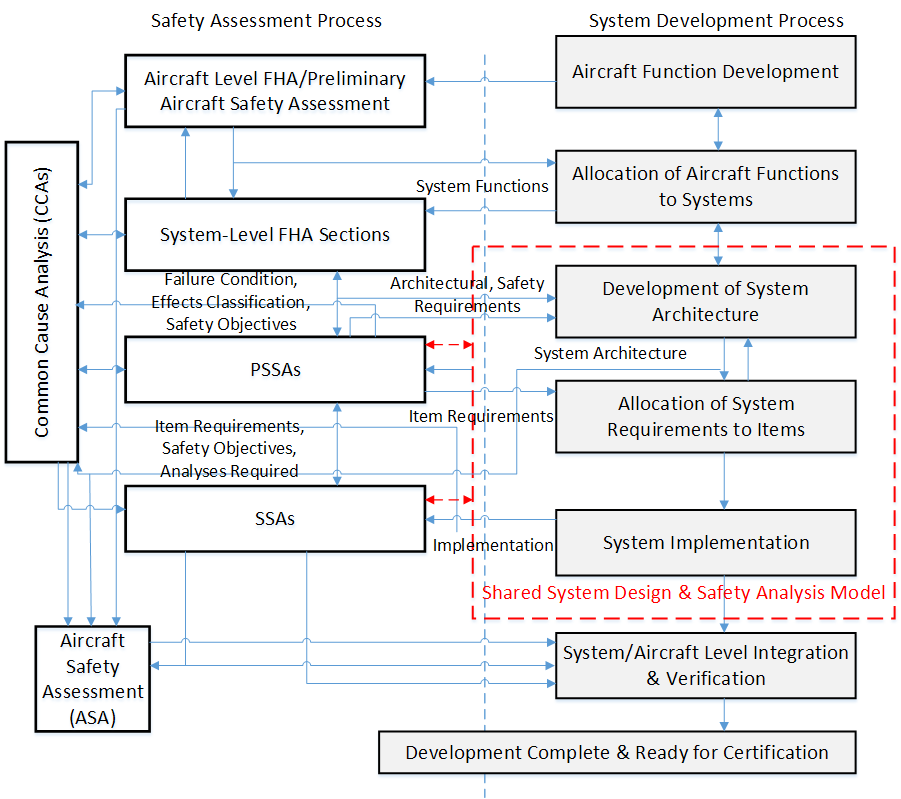
\includegraphics[width=1.0\textwidth]{images/Safety_Assessment_Process.png}
	%\vspace{-0.4in}
	\caption{Using the Shared System/Safety Model in the ARP4754A Safety Assessment Process}
	\label{fig:proposed_safety_process}
\end{figure*}

The safety assessment process is part of the development life cycle, and is tightly coupled with the system development and verification processes. It is used to show compliance with certification requirements and for meeting a company's internal safety standards. The guidelines presented in ARP4761 include various industry accepted safety assessment practices. They are summarized here for convenience. 

\begin{itemize}
\item Functional Hazard Assessment (FHA): This process examines aircraft and system functions to identify potential functional failures and classifies the hazards associated with specific failure conditions. This is usually developed early in the development process and is updated throughout. 

\item Preliminary System Safety Assessment (PSSA): This will establish the system safety requirements and provide some indication that the system architecture can meet those safety requirements. This is also updated throughout the development process.

\item System Safety Assessment (SSA): This process collects, analyzes, and documents verification that the system, as implemented, meets the safety requirements established by the PSSA. 

\item Common Cause Analysis (CCA): The CCA establishes physical and functional separation, isolation, and independence requirements between systems and verifies that these requirements have been met.
\end{itemize}

As shown in Figure~\ref{fig:proposed_safety_process}, these processes occur during the development process and are continually updated throughout. The safety engineers then use the acquired understanding to conduct safety analysis, construct the safety analysis artifacts, and compare the analysis results with established safety objectives and safety-related requirements. 

In practice, prior to performing the safety assessment of a system, the safety engineers are often equipped with the domain knowledge about the system, but do not necessarily have detailed knowledge of how the software functions are designed. Acquiring the required knowledge about the behavior and implementation of each software function in a system can be time-consuming. Industry practitioners have come to realize the benefits and importance of using models to assist the safety assessment process (either by augmenting the existing system design model, or by building a separate safety model), and a revision of the ARP4761 to include model based safety analysis is under way. Capturing failure modes in models and generating safety analysis artifacts directly from models could greatly improve communication and synchronization between system designer and safety engineers, and provide the ability to more accurately analyze complex systems. 

A single unified model to conduct both system development and safety analysis can help reduce the gap in comprehending the system behavior and transferring the knowledge between the system designers and the safety analysts. This maintains a living model that captures the current state of the system design as it moves through the system development lifecycle.

A single unified model also allows all participants of the ARP4754A process to be able to communicate and review the system design using a ``single source of truth.''

A model that supports both system design and safety analysis must describe both the system design information (e.g., system architecture, functional behavior) and safety-relevant information (e.g., failure modes, failure rates).  It must do this in a way that keeps the two types of information distinguishable, yet allows them to interact with each other.

Figure~\ref{fig:proposed_safety_process} presents our proposed use of this shared system design and safety analysis model in the context of the ARP4754A Safety Assessment Process Model (derived from Figure 7 of ARP4754A). The shared model is one of the system development artifacts from the ``Development of System Architecture'' and ``Allocation of System Requirements to Item'' activities in the System Development Process, which interacts with the PSSAs and SSAs activities in the Safety Assessment Process. This is seen as a box labeled ``Shared System Design and Safety model'' on the right column of the figure. The shared model can serve as an interface to capture the information from the system design and implementation that is relevant for the safety analysis.






%	\subsection{Safety Critical Systems}
\label{sec:SA_background}
A safety critical system is a system whose safety cannot be shown solely by test, whose logic is difficult to comprehend without the aid of analytical tools, and whose failure can directly or indirectly cause significant loss of life or property\cite{SAE:ARP4761}. Guaranteeing safety and reliability of safety critical systems is mandatory. The process that guides this guarantee is highly standardized and controlled~\cite{RTCA:StdC,SAE:ARP4761} . Due to the complexity of critical systems, the field of safety analysis has in recent decades turned to formal methods~\cite{mattarei,Bozzano:2010:DSA:1951720}. In practice, a systems behavior can be described in a variety of ways that include diagrams, textual descriptions, and operational procedures~\cite{SAE:ARP4754A}. These descriptions must be clear and well defined in order to avoid ambiguous interpretation. The formal definition of system behavior has a unique interpretation and is therefore a good candidate for automated analysis in order to validate requirements and spot design flaws~\cite{Joshi05:Dasc}. 

Model checking is a technique used to allow exhaustive and automatic checking of whether a system model (formal system definition) meets a set of formal requirements. As early as the '90's, using model checking for safety requirements began to surface in the critical systems literature\cite{DBLP:conf/safecomp/CimattiGMRTT98,DBLP:conf/edcc/BernardeschiFGM96}. Current tools in safety analysis use model checking techniques during the development and assessment of safety critical systems, \cite{mattarei,CAV2015:BoCiGrMa,symbAltaRica,DBLP:conf/tacas/BittnerBCCGGMMZ16}.







%	\subsection{Model Based Safety Analysis}
\label{sec:mbsa}

Safety engineers traditionally perform safety analysis based on information synthesized from a variety of sources including informal design models and requirement documents. These analyses are highly subjective and dependent on the skill of the analyst. The lack of precise models requires the analyst to devote a fair amount of time to information gathering of the architecture and behavior of the system. On the other hand, in Model Based Safety Aanalysis (MBSA), the system and safety engineers share a common system model created using the model based development process. By extending the system model and relevant physical control systems, automated support can be provided for much of the safety analysis. Using a common model for both system and safety engineering and automating parts of safety analysis assists in the reduction of cost and improves the quality of the safety analysis, but this is not without disadvantages if the model itself is faulty. 

In model based system development, various development activities such as simulation, verification, testing, and code generation are based on a formal model of the system under development\cite{Joshi05:Dasc}. This is called the nominal model. Model based development was extended to include model based safety analysis\cite{Joshi05:Dasc,Joshi05:SafeComp,Joshi07:Hase,DBLP:conf/cav/BozzanoCPJKPRT15,CAV2015:BoCiGrMa,info17:HaLuHo}. The goal of MBSA is to incorporate safety analysis into the model based development process in order to provide information on the safety of the formal model of the system under development. In this process, the nominal (non-failure) system behavior that is captured in the model based development process is augmented with the fault behavior of the system. Model based safety analysis then operates on a formal model that describes both nominal system behavior and the fault model, which describes fault behavior. 






%	\subsection{Safety Assessment Process}
\label{subsec:process}

ARP4761, the Guidelines and Methods for Conducting Safety Assessment Process on Civil Airborne Systems and Equipment, provides guidance on applying development assurance at each hierarchical level throughout the development life cycle of highly-integrated/complex aircraft systems, and has been recognized by the Federal Aviation Administration (FAA) as an acceptable method to establish the assurance process~\cite{SAE:ARP4761}.

\begin{figure*}[h!]
	%\vspace{-0.956in}
	\centering
	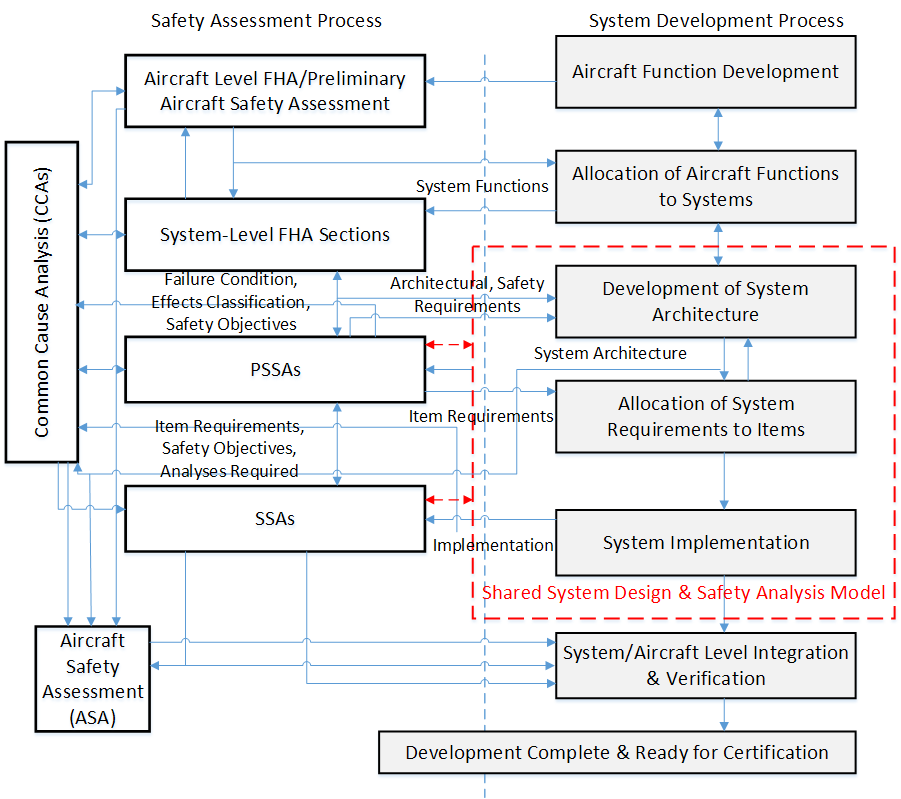
\includegraphics[width=1.0\textwidth]{images/Safety_Assessment_Process.png}
	%\vspace{-0.4in}
	\caption{Using the Shared System/Safety Model in the ARP4754A Safety Assessment Process}
	\label{fig:proposed_safety_process}
\end{figure*}

The safety assessment process is part of the development life cycle, and is tightly coupled with the system development and verification processes. It is used to show compliance with certification requirements and for meeting a company's internal safety standards. The guidelines presented in ARP4761 include various industry accepted safety assessment practices. They are summarized here for convenience. 

\begin{itemize}
\item Functional Hazard Assessment (FHA): This process examines aircraft and system functions to identify potential functional failures and classifies the hazards associated with specific failure conditions. This is usually developed early in the development process and is updated throughout. 

\item Preliminary System Safety Assessment (PSSA): This will establish the system safety requirements and provide some indication that the system architecture can meet those safety requirements. This is also updated throughout the development process.

\item System Safety Assessment (SSA): This process collects, analyzes, and documents verification that the system, as implemented, meets the safety requirements established by the PSSA. 

\item Common Cause Analysis (CCA): The CCA establishes physical and functional separation, isolation, and independence requirements between systems and verifies that these requirements have been met.
\end{itemize}

As shown in Figure~\ref{fig:proposed_safety_process}, these processes occur during the development process and are continually updated throughout. The safety engineers then use the acquired understanding to conduct safety analysis, construct the safety analysis artifacts, and compare the analysis results with established safety objectives and safety-related requirements. 

In practice, prior to performing the safety assessment of a system, the safety engineers are often equipped with the domain knowledge about the system, but do not necessarily have detailed knowledge of how the software functions are designed. Acquiring the required knowledge about the behavior and implementation of each software function in a system can be time-consuming. Industry practitioners have come to realize the benefits and importance of using models to assist the safety assessment process (either by augmenting the existing system design model, or by building a separate safety model), and a revision of the ARP4761 to include model based safety analysis is under way. Capturing failure modes in models and generating safety analysis artifacts directly from models could greatly improve communication and synchronization between system designer and safety engineers, and provide the ability to more accurately analyze complex systems. 

A single unified model to conduct both system development and safety analysis can help reduce the gap in comprehending the system behavior and transferring the knowledge between the system designers and the safety analysts. This maintains a living model that captures the current state of the system design as it moves through the system development lifecycle.

A single unified model also allows all participants of the ARP4754A process to be able to communicate and review the system design using a ``single source of truth.''

A model that supports both system design and safety analysis must describe both the system design information (e.g., system architecture, functional behavior) and safety-relevant information (e.g., failure modes, failure rates).  It must do this in a way that keeps the two types of information distinguishable, yet allows them to interact with each other.

Figure~\ref{fig:proposed_safety_process} presents our proposed use of this shared system design and safety analysis model in the context of the ARP4754A Safety Assessment Process Model (derived from Figure 7 of ARP4754A). The shared model is one of the system development artifacts from the ``Development of System Architecture'' and ``Allocation of System Requirements to Item'' activities in the System Development Process, which interacts with the PSSAs and SSAs activities in the Safety Assessment Process. This is seen as a box labeled ``Shared System Design and Safety model'' on the right column of the figure. The shared model can serve as an interface to capture the information from the system design and implementation that is relevant for the safety analysis.



%	\section{Related Work}
\label{sec:related_work}
Minimal cut sets generated by monolithic analysis look only at explicitly defined faults throughout the architecture and attempt through various techniques to find the minimal violating set for a particular property. We outline some of the common monolithic approaches to minimal cut set generation in this section.

The representation of Boolean formulae as Binary Decision Diagrams (BDDs) was first formalized in the mid 1980s~\cite{bryant1986graph} and were extended to the representation of fault trees not many years later~\cite{rauzy1993new}. After this formalization, the BDD approach to FTA provided a new approach to safety analysis. The model is constructed using a BDD, then a second BDD - usually slightly restructured - is used to encode MinCutSets~\cite{rauzy2008binary}. Unfortunately, due to the structure of BDDs, the worst case is exponential in size in terms of the number of variables~\cite{bryant1986graph,rauzy1993new,rauzy2008binary}. In industrial sized systems, this is not realistically useful. 

SAT based computation was then introduced to address scalability problems in the BDD approach; initially it was used as a preprocessing step to simplify the decision diagram~\cite{bozzano2015safety}, but later extended to allow for all MinCutSet processing and generation without the use of BDDs~\cite{bozzano2015efficient}. Since then, numerous safety related research groups have focused on leveraging the power of model checking in the problems of safety assessment~\cite{bieber2002combination,schafer2003combining,bozzano2007symbolic,bozzano2003improving,volk2017fast,Joshi05:SafeComp,bozzano2015efficient,stewart2020safety}. 

Bozzano et al. formulated a Bounded Model Checking (BMC) approach to the problem by successively approximating the cut set generation and computations to allow for an ``anytime approximation" in cases when the cut sets were simply too large and numerous to find~\cite{bozzano2015efficient,mattarei2016scalable}. These algorithms are implemented in xSAP~\cite{DBLP:conf/tacas/BittnerBCCGGMMZ16} and COMPASS~\cite{compass30toolset}. 

The model based safety assessment tool AltaRica 3.0~\cite{prosvirnova:tel-01119730} performs a series of processing to transform the model into a reachability graph and then compile to Boolean formula in order to compute the MinCutSets~\cite{prosvirnova2015automated}. Other tools such as HiP-HOPS~\cite{papadopoulos2001model} have implemented algorithms that follow the failure propagations in the model and collect information about safety related dependencies and hazards. The Safety Analysis Modeling Language (SAML)~\cite{Gudemann:2010:FQQ:1909626.1909813} provides a safety specific modeling language that can be translated into a number of input languages for model checkers in order to provide model checking support for MinCutSet generation.

To our knowledge, a fully compositional approach to calculating minimal cut sets has not been introduced.





















\section{The Safety Annex}
\label{sec:safety_annex}

In this section, we describe the main features and functionality of the Safety Annex. The usage of the terms error, failure, and fault follow their definitions in Section~\ref{sec:terminology}. We use {\em fault} as the generic modeling keyword throughout the AADL model hierarchy.

The Safety Annex Users Guide can be found at \url{https://github.com/loonwerks/AMASE/tree/develop} along with the tool plugins and examples described in this report. 

\subsection{Modeling Language for System Design}
\label{subsec:aadl}
We are using the Architectural Analysis and Design Language (AADL) to construct system architecture models~\cite{FeilerModelBasedEngineering2012}.  AADL is an SAE International standard that defines a language and provides a unifying framework for describing the system architecture for ``performance-critical, embedded, real-time systems''~\cite{AADL_Standard}. From its conception, AADL has been designed for the design and construction of avionics systems.  Rather than being merely descriptive, AADL models can be made specific enough to support system-level code generation.  Thus, results from analyses conducted, including the new safety analysis proposed here, correspond to the system that will be built from the model.  

An AADL model describes a system in terms of a hierarchy of components and their interconnections, where each component can either represent a logical entity (e.g., application software functions, data) or a physical entity (e.g., buses, processors). An AADL model can be extended with language annexes to provide a richer set of modeling elements for various system design and analysis needs (e.g., performance-related characteristics, configuration settings, dynamic behaviors). The language definition is sufficiently rigorous to support formal analysis tools that allow for early phase error/fault detection.






\subsection{Modeling Language for System Design}
\label{subsec:aadl-agree}
We are using the Architectural Analysis and Design Language (AADL)~\cite{FeilerModelBasedEngineering2012} to construct system architecture models.  AADL is an SAE International standard that defines a language and provides a unifying framework for describing the system architecture for ``performance-critical, embedded, real-time systems''~\cite{AADL_Standard}. From its conception, AADL has been designed for the design and construction of avionics systems.  
Rather than being merely descriptive, AADL models can be made specific enough to support system-level code generation.  Thus, results from analyses conducted, including the new safety analysis proposed here, correspond to the system that will be built from the model.  

An AADL model describes a system in terms of a hierarchy of components and their interconnections, where each component can either represent a logical entity (e.g., application software functions, data) or a physical entity (e.g., buses, processors). An AADL model can be extended with language annexes to provide a richer set of modeling elements for various system design and analysis needs (e.g., performance-related characteristics, configuration settings, dynamic behaviors). The language definition is sufficiently rigorous to support formal analysis tools that allow for early phase error/fault detection.

The Assume Guarantee Reasoning Environment (AGREE)~\cite{NFM2012:CoGaMiWhLaLu} is a tool for formal analysis of behaviors in AADL models.  It is implemented as an AADL annex and annotates AADL components with formal behavioral contracts. Each component's contracts can include assumptions and guarantees about the component's inputs and outputs respectively, as well as predicates describing how the state of the component evolves over time. AGREE translates an AADL model and the behavioral contracts into Lustre~\cite{Halbwachs91:IEEE} and then queries a user-selected
model checker to conduct the back-end analysis. The analysis %is
can be performed compositionally following the architecture hierarchy such that analysis at a higher level is based on the components at the next lower level.  When compared to monolithic analysis (i.e., analysis of the flattened model composed of all components), the compositional approach allows the analysis to scale to much larger systems~\cite{NFM2012:CoGaMiWhLaLu}. 

%In the avionics context, the software functions/applications, the hardware equipment, and the system that is composed of their integration can all be represented as components connected to/composed of/bind to other components in a hierarchical AADL model. AGREE contracts can be used to capture the functional requirements at each level of the hierarchy. Once the model has been reviewed and the requirements captured have been validated, the back-end analysis can be conducted to verify if each level of the model implements its higher level requirements correctly.

%AADL with the AGREE extension serves as a good candidate as the modeling language for describing the system design aspects of a shared system design and safety analysis model. 
In our prior work~\cite{Stewart17:IMBSA}, we added an initial failure effect modeling capability to the AADL/AGREE language and tool set.  We are continuing this work so that our tools and methodology can be used to satisfy system safety objectives of ARP4754A and ARP4761.  

\begin{comment}
In particular, our goals are to:

\begin{itemize}
	\item Provide a comprehensive, qualitative description of the causal relationship between basic failure events and system level safety requirements.
	\item Provide an accurate, quantitative description of the contribution relationship between failure rates of the fault tree basic events and numerical probability requirements at the system level.
\end{itemize}
\end{comment}
%The remainder of the paper describes our approach towards both of the goals.





\subsection{Basic Functionality of the Safety Annex}

An AADL model of the nominal system behavior specifies the hardware and software components of the system and their interconnections. This nominal model is then annotated with assume-guarantee contracts using the AGREE annex for AADL. The nominal model requirements are verified using compositional verification techniques based on inductive model checking~\cite{2017arXiv171201222G}.

Once the nominal model behavior is defined and verified, the Safety Annex can be used to specify possible faulty behaviors for each component. The faults are defined on each of the relevant components using a customizable library of fault nodes and the faults are assigned a probability of occurrence. A probability threshold is also defined at the system level. This extended model can be analyzed to verify the behavior of the system in the presence of faults. Verification of the nominal model with or without the fault model is controlled through the safety analysis option during AGREE verification.

To illustrate the syntax of the Safety Annex, we use an example based on the Wheel Brake System (WBS) described in AIR6110 standards document and used in  previous work ~\cite{Stewart17:IMBSA, AIR6110}.

The \textit{fault library} contains commonly used fault node definitions. Commonly used faults in various systems include \textit{fail\_to} fault, where the output of a component fails to a particular value, for instance a pump may fail to produce any output and hence the fail to value is zero. Another example of a commonly occuring fault is an \textit{inverted\_boolean}. For example, a sensor may have an inverted value fault present on its boolean output. The fault library is simply a collection of fault nodes with these commonly used fault definitions which are then easily referenced within the fault definitions in the safety annex. 


A \textit{fault declaration} is shown in Figure~\ref{fig:fault_pump}. This describes a fail to zero fault in a pump. The \textit{fail\_to} node provides the mechanism in which a faulty value is injected into the fault model. When the \textit{trigger} condition for this pump fault is satisfied, the nominal component output value is overridden by the failure value. In this particular example, the pump will fail to produce any pressure and the hydraulic fluid ceases being pumped through the lines.  

\begin{figure*}[h!]
	\vspace{-0.6in}
	\begin{center}
		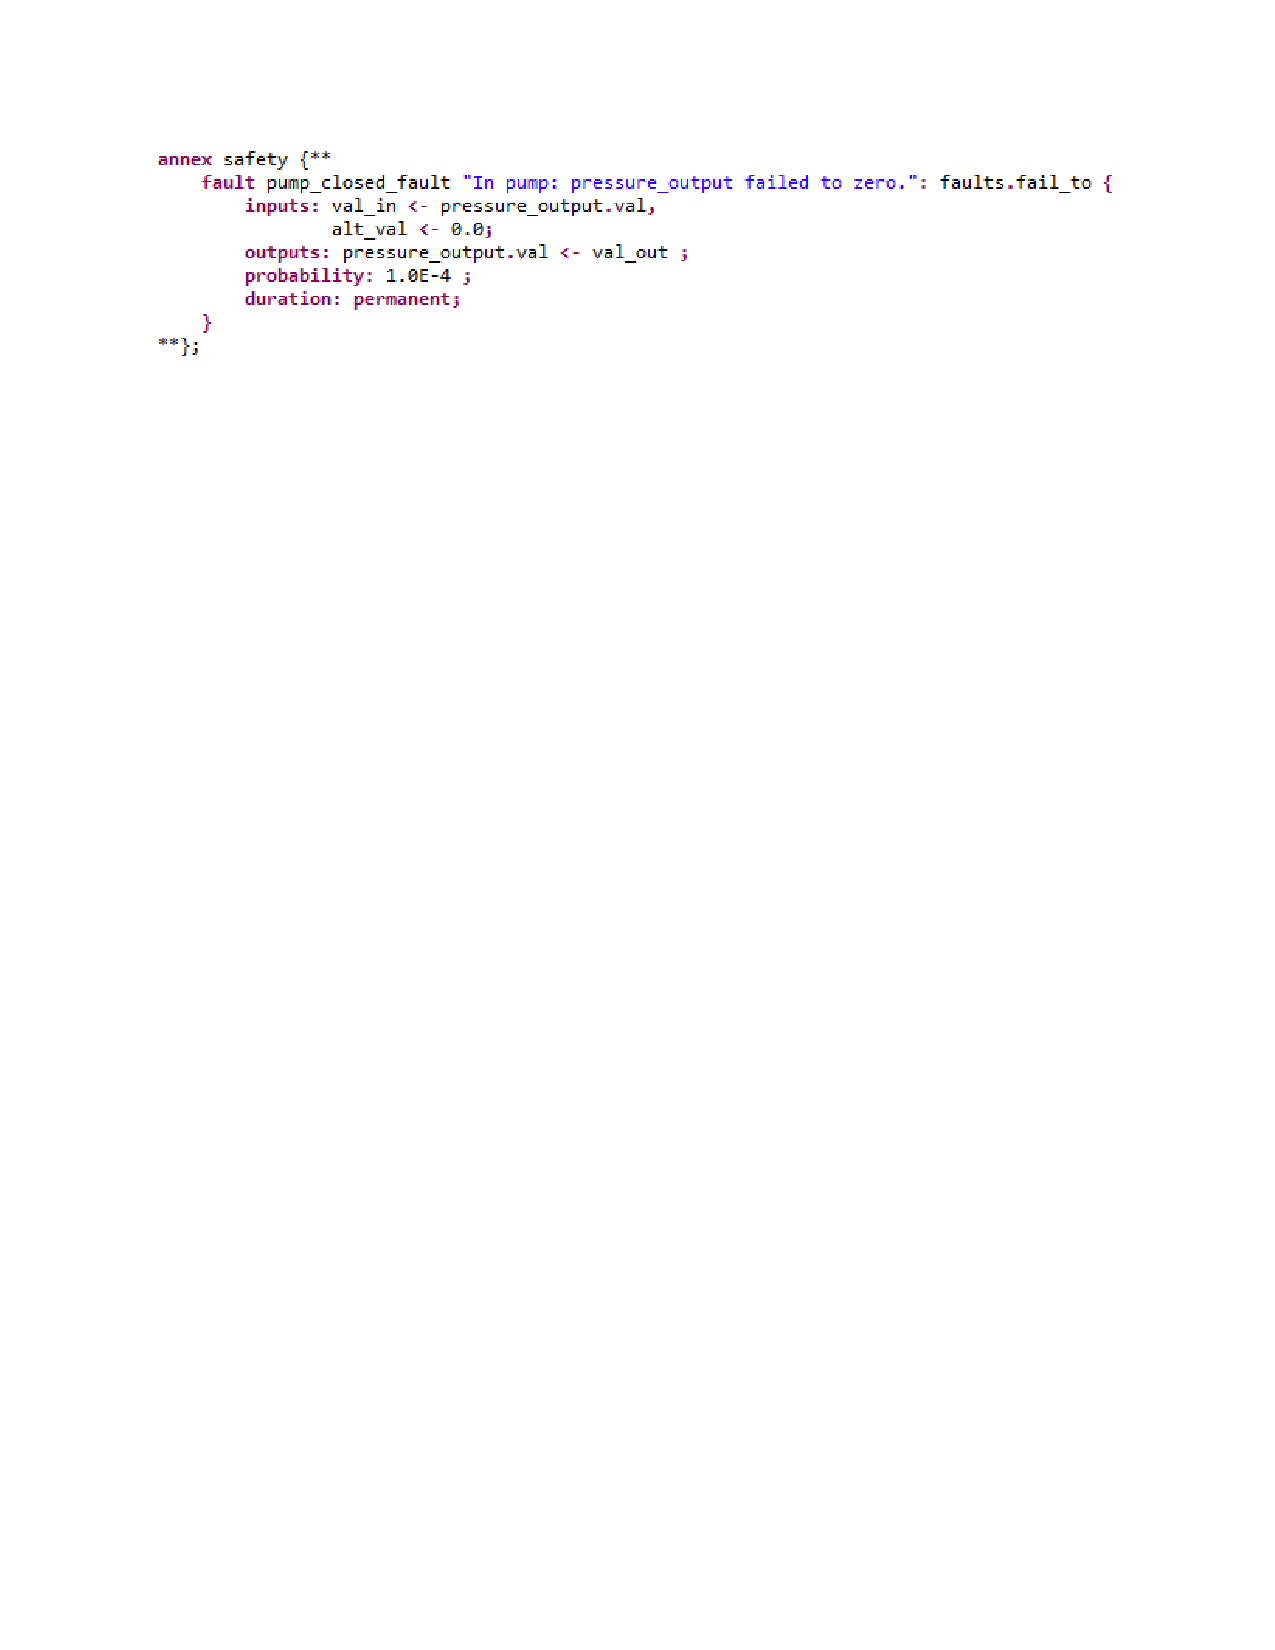
\includegraphics[trim=30 635 0 30,clip,width=1.3\dimexpr\textwidth-1.5cm\relax]{images/pump_fault.pdf}
		\caption{Pump Fault Definition in the Safety Annex}
		\label{fig:fault_pump}
	\end{center}
\end{figure*}

The \textit{fault statement} consists of a unique description string, the fault node definition name, and a series of \textit{fault subcomponent} statements. Contents of the fault statement are as follows.\\
\textbf{Inputs} in a fault statement are the parameters of the fault node definition. In the example above, \textit{val\_in} and \textit{alt\_val} are the two input parameters of the fault node. These are linked to the output from the Pump component (\textit{pressure\_output.val}), and \textit{alt\_value}, a fail to value of zero. When the analysis is run, these values are passed into the fault node definition.\\
\textbf{Outputs} of the fault definition correspond to the outputs of the fault node. The fault output statement links the component output (\textit{pressure\_output.val}) with the fault node output (\textit{val\_out}). If the fault is triggered, the nominal value of \textit{pressure\_output.val} is overridden by the failure value output by the fault node. Faulty outputs can take deterministic or non-deterministic values. \\
\textbf{Probability} (optional) describes the probability of a fault occurrence.\\
\textbf{Duration} describes the duration of the fault; currently the Safety Annex supports permanent faults.\\

\subsection{Hardware Failures and Dependent Faults}

Failures in hardware (HW) components can trigger behavioral faults in the software (SW) or system (SYS) components that depend on them.  For example, a CPU failure may trigger faulty behavior in threads bound to that CPU. In addition, a failure in one HW component may trigger failures in other HW components located nearby, such as cascading failure caused by a fire or water damage.

Faults propagate in AGREE as part of the nominal behavior of a system. This means that any propagation in the HW portion of an AADL model would have to be artificially modeled using data ports and AGREE behaviors in SW. This is less than ideal as there may not be concrete behaviors associated with HW components. In other words, faulty behaviors mainly manifest themselves on the software components that depend on the hardware components.

To better model faults at the system level dependent on HW failures, there is a fault definition specifically designed for HW components. In comparison to the basic fault statement introduced in the previous section, users are not specifying behavioral effects for the HW failures, nor data ports to apply the failure. An example of a hardware component fault declaration is shown in Figure~\ref{fig:hardware_fault}.

\begin{figure}[h!]
	\begin{center}
		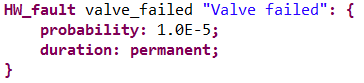
\includegraphics[width=.4\textwidth]{images/hw_fault.png}
		\caption{Hardware Fault in the Safety Annex}
		\label{fig:hardware_fault}
	\end{center}
\end{figure}

%\noindent
%\begin{minipage}{\textwidth}% to keep image and caption on one page
%\makebox[\linewidth]{%        to center the image
%  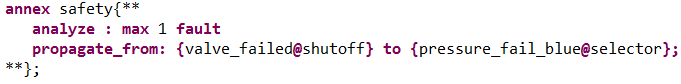
\includegraphics[keepaspectratio=true,scale=0.6]{images/fault_propagation.png}}
%\captionof{figure}{Fault Propagation}
%\label{fig:fault_propagation}%      only if needed  
%\end{minipage}

\begin{figure*}[]
	\begin{center}
		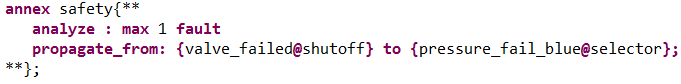
\includegraphics[width=.7\textwidth]{images/fault_propagation.png}
		\caption{Fault Propagation}
		\label{fig:fault_propagation}
	\end{center}
\end{figure*}

When analyzing hardware specific faults, it is often of interest to see how these faults may propagate to other components of the system, specifically the software components. As an example, consider software systems that run on a particular CPU. This CPU has a hardware fault pertaining to overheating. An important question is how this hardware specific fault may propagate to components that rely on the CPU. In the nominal model, there is a binding between hardware and software components in AADL that is specified within the system implementation. In order to model this type of fault, users can specify fault dependencies in the system implementation where these dependencies are clearly defined. This is the only case of explicit fault propagation within the Safety Annex and in this case the propagation only is from the hardware to the software that runs on it. An example of a fault dependency specification is shown in Figure~\ref{fig:fault_propagation}, showing that a valve failure triggers a pressure failure fault at a subcomponent that relies upon that valve. 


\subsection{Implementation Details}

\begin{figure*}[h!]
\begin{center}
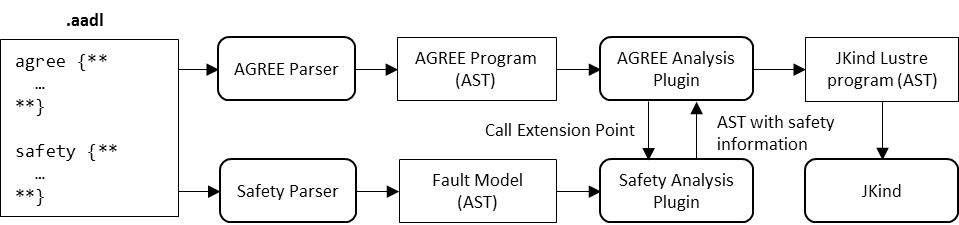
\includegraphics[width=.9\textwidth]{images/arch.png}
\vspace{0.1in}
\caption{Safety Annex Plug-in Design}
\label{fig:plugin-arch}
\end{center}
\end{figure*}

This section provides an overview of how the Safety Annex is related to AADL, AGREE, and the JKind model checker.  The Safety Annex is written in Java as a plug-in for the OSATE AADL toolset, which is built on Eclipse.  It is not designed as a stand-alone extension of the language, but works with behavioral contracts specified AGREE annex and associated tools.  AGREE allows assume-guarantee behavioral contracts to be added to AADL components.  The language used for contract specification is based on the Lustre dataflow language~\cite{Halbwachs91:IEEE}. 

The organization of these interactions  is shown in Figure~\ref{fig:plugin-arch}. The AADL file is annotated with AGREE contracts which creates the nominal model. This nominal model is parsed and sent to JKind where formal verification is performed. If the Safety Annex is also annotated within this model, this creates the extended (fault) model. When desired, the user can run ``Perform Safety Analysis'' within the Osate environment. This creates an extension point where the Safety Analysis informaiton is added into the AGREE model before getting passed to JKind for analysis. In either case, the JKind verification result is returned and displayed to the user in the Osate environment. For more information about this process or figures depicting the environment and analysis results, see the Safety Annex Users Guide or the Safety Annex Technical Report~\cite{amaseRepo, SATechReport}.



%AGREE contracts are used to define the nominal behaviors of system components as {\em guarantees} that hold when {\em assumptions} about the values the component's environment are met.  The Safety Annex extends these contracts to allow faults to modify the behavior of component inputs and outputs.  To support these extensions, AGREE implements an Eclipse extension point interface that allows other plug-ins to modify the generated abstract syntax tree (AST) prior to its submission to the solver.  If the Safety Annex is enabled, these faults are added to the AGREE contract and, when triggered, override the nominal guarantees provided by the component.  An example of a portion of an initial AGREE node and its extended contract is shown in Figure~\ref{fig:comp}.  The \texttt{\_\_fault} variables and declarations are added to allow the contract to override the nominal behavioral constraints (provided by guarantees) on outputs.  In the Lustre language, \texttt{assertion}s are constraints that are assumed to hold in the transition system.

%\begin{figure}
%\vspace{-0.1in}
%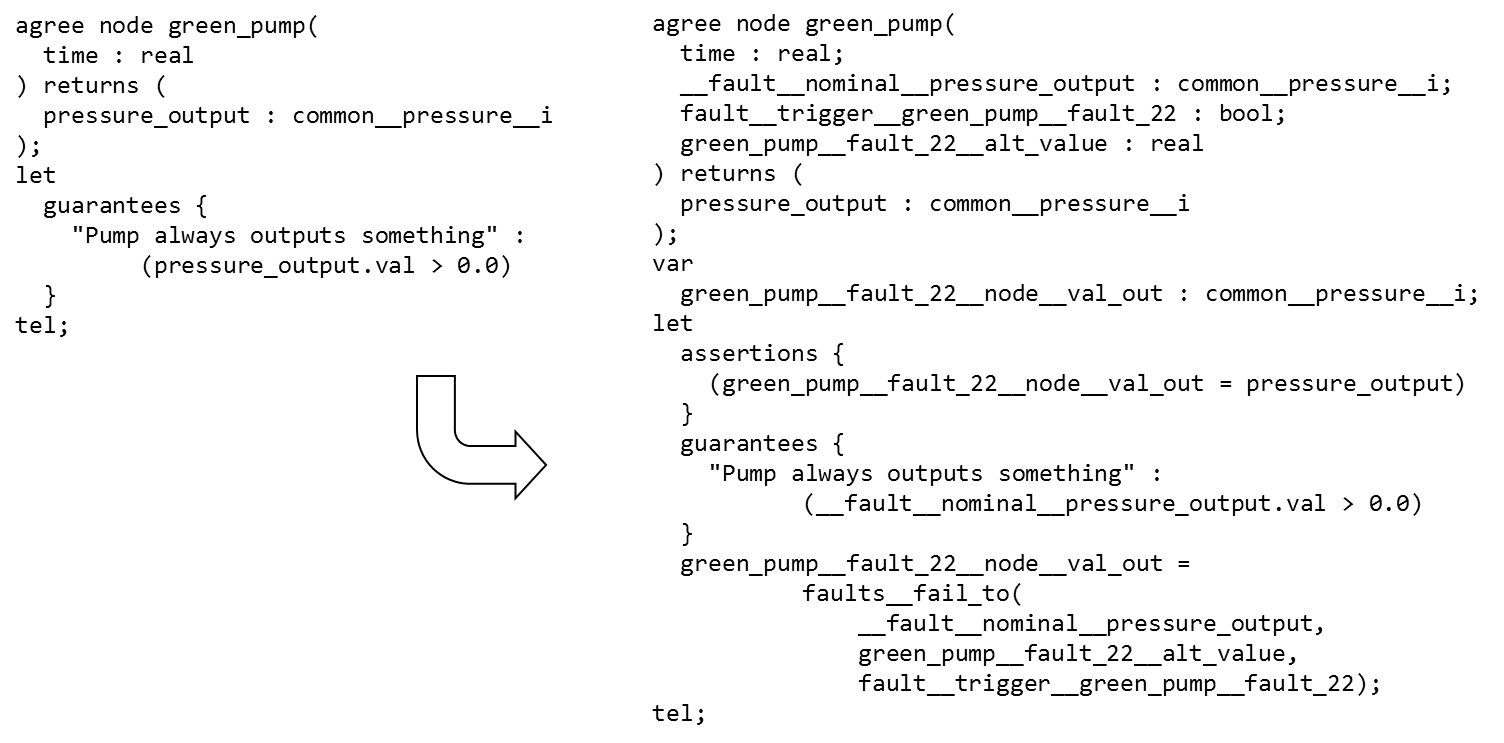
\includegraphics[width=\textwidth]{images/sample_code.png}
%\vspace{-0.3in}
%\caption{Nominal AGREE node and its extension with faults}
%\label{fig:comp}
%\end{figure}

%An annotation in the AADL model determines the fault hypothesis.  This may specify either a maximum number of faults that can be active at any point in execution (typically one or two), or that only faults whose probability of simultaneous occurrence is above some probability threshold should be considered.  In the former case, we assert that the sum of the true {\em fault\_\_trigger} variables is below some integer threshold.  In the latter, we determine all  combinations of faults whose probabilities are above the specified probability threshold, and describe this as a proposition over {\em fault\_\_trigger} variables.

%Once augmented with fault information, the AGREE model follows the standard AGREE translation path to the model checker JKind~\cite{2017arXiv171201222G}, an infinite-state model checker for safety properties.  The augmentation includes traceability information so that when counterexamples are displayed to users, the active faults for each component are visualized.




 \section{Case Studies}
\label{sec:case_study}
To demonstrate the effectiveness of the Safety Annex, we describe two case studies.

\begin{figure*}[!ht]
	\begin{center}
		%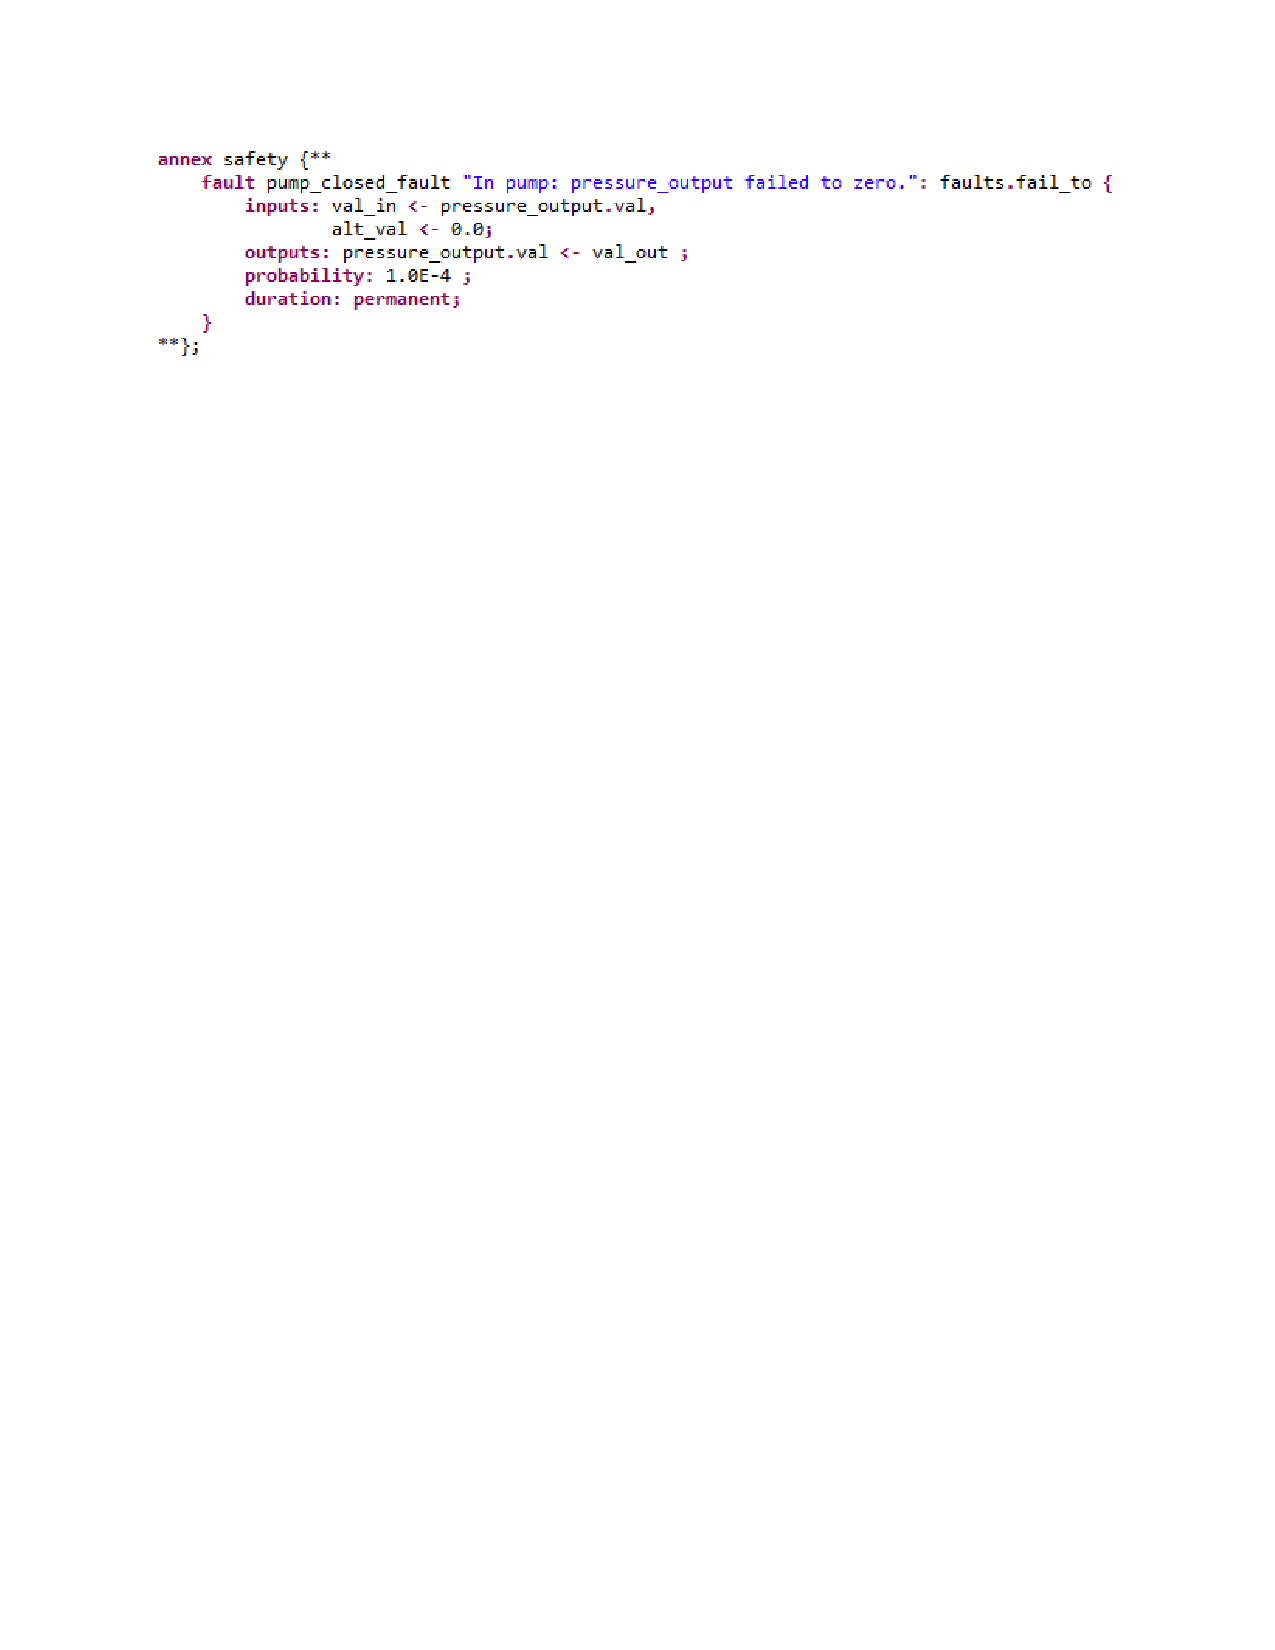
\includegraphics[trim=0 330 150 0,clip,width=1.0\textwidth]{images/pump_fault.png}
		\vspace{-50pt}
		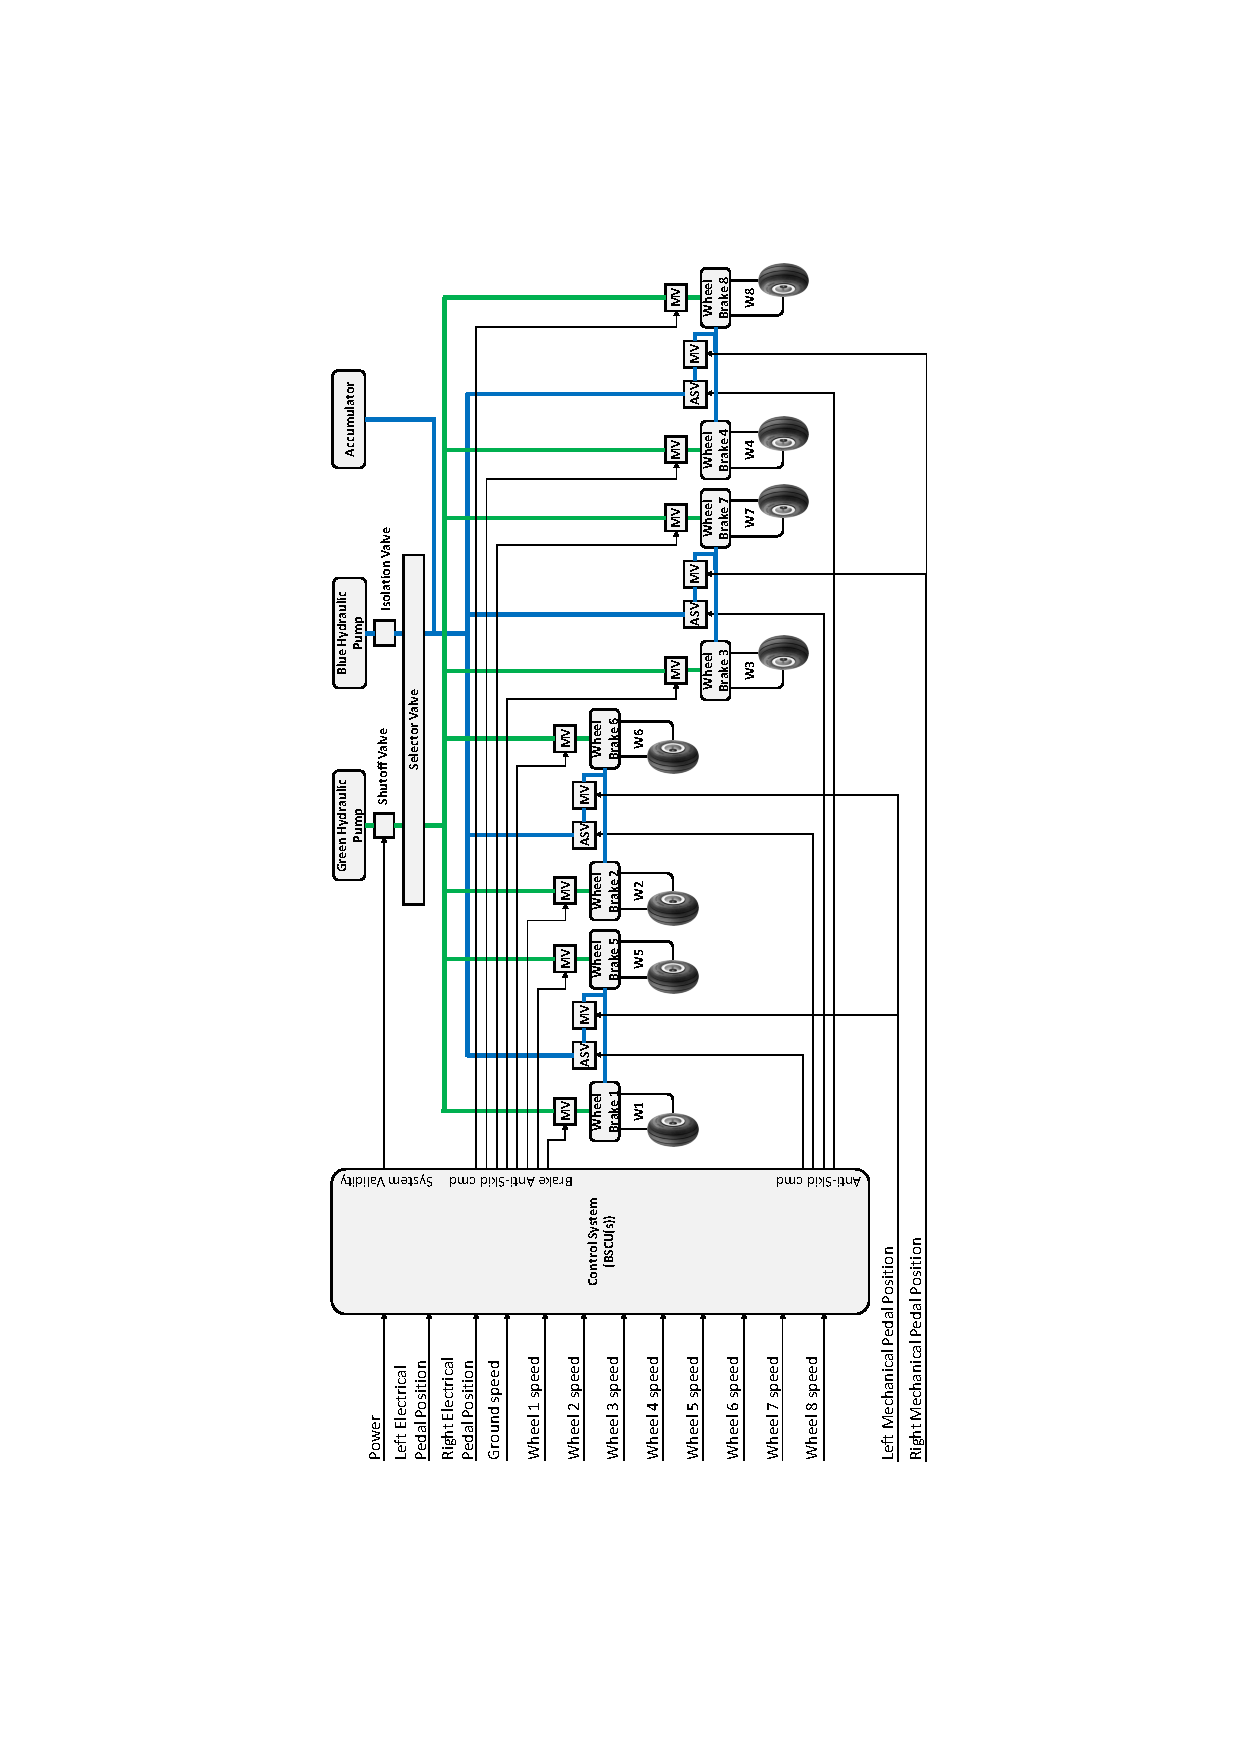
\includegraphics[trim=20 20 20 20,clip,width=1.0\textwidth]{images/wbs_large.pdf}
		\vspace{-70pt}
		\caption{High level Wheel Brake System}
 		\label{fig:wbs1}
	\end{center}
\end{figure*}

\subsection{Wheel Brake System}
The Wheel Brake System (WBS) described in AIR6110~\cite{AIR6110} is a well-known example that has been used as a case study for safety analysis, formal verification, and contract based design~\cite{DBLP:conf/cav/BozzanoCPJKPRT15, 10.1007/978-3-319-11936-6-7, CAV2015:BoCiGrMa, Joshi05:SafeComp, mattarei}. The preliminary work for the safety annex used a simplified model of the WBS~\cite{Stewart17:IMBSA}. In order to demonstrate scalability of our tools and compare results with other studies, a functionally and structurally equivalent AADL version was constructed of one of the most complex WBS xSAP models (arch4wbs)~\cite{DBLP:conf/cav/BozzanoCPJKPRT15}. 

The Aerospace Information Report 6110 (AIR6110) document provides an example of a single aircraft system, namely the braking system, for the hypothetical passenger aircraft model S18. The two engine passenger aircraft is designated to carry up to 350 passengers for an average flight time of 5 hours. The purpose of the system is to provide a clear example of systems development and its analysis using the methods and tools described in ARP4754A/ED-79A. This brake system implements the aircraft function \textit{''Decelerate aircraft on the ground (stopping on the runway)"}. The wheel brake system architecture is shown in Figure~\ref{fig:wbs1} and is taken from the work of Mattarei~\cite{mattarei}. 

\subsubsection{WBS overview and architecture description}
The WBS is a hydraulic braking system that provides braking of left and right landing gears, each of which have four wheels. Each landing gear can be individually controlled by the pilot through left/right brake pedals. 

The WBS is composed of two main parts: the control system and the physical system. The control system electronically controls the physical system and contains a redundant Braking System Control Unit (BSCU) in case of failure. In addition to the redundant BSCU channel, the control system is composed of a number of logical components including sensors for the wheels and brake pedal position, a monitor system that checks validity of the BSCU channel, and the command system which commands braking for each of the 8 wheels. The control system is primarily used in the normal mode of operation to command brake pressure.  

The physical system consists of the hydraulic circuits running from hydraulic pumps to wheel brakes. This circuit contains the pumps for both normal and alternate modes of operation (named green and blue lines respectively), a selector valve which selects the circuit depending on input from the BSCU, meter valves at each wheel. These are the physical components that provide braking force to the 8 wheels of the aircraft.

There are three operating modes in the WBS model. In \textit{normal} mode, the system uses the \textit{green} hydraulic circuit. In the normal mode of operation, the selector valve uses the green hydraulic pump to supply fluid to the wheels. Each of the 8 wheels has one meter valve which  are controlled through electronic commands coming from the BSCU. These signals provide brake commands as well as antiskid commands for each of the wheels. The braking command is determined through a sensor on the pilot pedal position. The antiskid command is calculated based on information regarding ground speed, wheel rolling status, and braking commands.

In \textit{alternate} mode, the system uses the \textit{blue} hydraulic circuit.  The wheels are all \textit{mechanically} braked in pairs (one pair per landing gear). The alternate system is composed of the blue hydraulic pump, four meter valves, and four antiskid shutoff valves. The meter valves are mechanically commanded through the pilot pedal corresponding to each landing gear. If the system detects lack of pressure in the green circuit, the selector valve switches to the blue circuit. This can occur if there is a lack of pressure from the green hydraulic pump, if the green hydraulic pump circuit fails, or if pressure is cut off by a shutoff valve. If the BSCU channel becomes invalid, the shutoff valve is closed.

The last mode of operation of the WBS is the \textit{emergency} mode. This is supported by the blue circuit but operates if the blue hydraulic pump fails. The accumulator pump has a reserve of pressurized hydraulic fluid and will supply this to the blue circuit in emergency mode.

The model contains 30 different kinds of components, 169 component instances, a model depth of 5 hierarchical levels.  The model includes one top-level assumption and  11 top-level system properties, with 113 guarantees allocated to subsystems.  There are a total of 33 different fault types and 141 fault instances within the model.  The large number of fault instances is due to the redundancy in the system design and its replication to control 8 wheels. 

An example property is to ensure no inadvertent braking of each of the 8 wheels.  This means that if all power and hydraulic pressure is supplied (i.e., braking is commanded), then either the aircraft is stopped (ground speed is zero), or the mechanical pedal is pressed, or brake force is zero, or the wheel is not rolling.


\subsubsection{Fault Analysis of WBS using Safety Annex}

Fault analysis on the top level WBS system was performed on the 11 top-level properties using two fault hypotheses.  In the first case, we allow at most one fault, and in the second we allow combinations of faults that exceed the acceptable probability for the top-level hazard defined in AIR6110.

We use this model to demonstrate the benefits of formal fault analysis and to show the scalability of our tools.  We applied both {\em monolithic} analysis, in which the entire model is flattened and analyzed at once, and also {\em compositional} analysis, where each architectural layer is analyzed hierarchically.
For the fault-free ``nominal'' system model, monolithic analysis requires 21 seconds, whereas compositional analysis requires 1 minute and 53 seconds.  Although the compositional time is longer, each sub-problem completes in less than 5 seconds.  The additional time for compositional analysis is  due to the start-up overhead to invoke the JKind model checker many times for individual layers.  On the other hand, when examining the model under a single-fault hypothesis (maximum one fault present in the system), compositional analysis requires 2 minutes 6 seconds, while monolithic analysis did not terminate after 60 minutes. The reason for this lies in the difference between compositional analysis and monolithic analysis as described in Section~\ref{subsec:agree}. 

Given a probabilistic fault hypothesis of $5*10^{-7}$, monolithic analysis requires 3 minutes 25 seconds.

During our analysis, we discovered that most properties were verified, but the \textit{Inadvertent braking at the wheel} properties are not resilient to a single fault nor do they meet the desired $10^{-9}$ fault threshold for probabilistic analysis.  In our model (as in the NuSMV model~\cite{DBLP:conf/cav/BozzanoCPJKPRT15}), there is a single pedal position sensor for the brake pedal.  If this sensor fails, it can command braking without a pilot request.  Given the counterexample returned by the tools, it is straightforward to diagnose the fault conditions that lead to property failure.

This counterexample can be used to further analyze the system design.  For our model, there are several possible reasons for failure: it could be that that redundant sensors are required on the pedals (here we note that the architecture of the pedal assembly is not discussed in AIR6110), or that the phase of flight is sufficiently short that we need to adjust our pedal failure rate to match this phase of flight, rather than normalizing the failure rate to per-flight-hour.  It is straightforward and computationally inexpensive to run the analysis, allowing quick iterations between systems and safety engineers. The sync and update between the preliminary system artifact analysis (FTA, etc.) and the architecture model continues until the system safety property is satisfied with the desired fault tolerance and failure probability achieved.

\subsection{Quad-Redundant Flight Control System}
\label{subsec:qrfc_case_study}
We have also used the Safety Annex to examine more complex fault types, such as {\em Byzantine} faults.  A Byzantine fault presents different symptoms to different observers, so that they may disagree regarding whether a fault is present. For example, a sensor may appear to be both failed and functional to different components to which it provides signal. 

The Quad-Redundant Flight Control System (QFCS) was first developed in Simulink and then manually translated in AADL by Backes, et. al. This system consists of four cross-checking flight control computers (FCC) as shown in Figure XX. The work done by Backus formalized the requirements for components of the system and for more detail on the requirements specification, see the original paper~\cite{QFCS15:backes}. 

The QFCS nominal system model was extended to model and analyze various types of faulty behaviors. Faulty behaviors were introduced to analyze the response of the system to multiple faults, and to evaluate fault mitigation logic in the model. As expected, the QFCS system-level properties failed when unhandled faulty behaviors were introduced.

We also used the Safety Annex to explore more complicated faults at the system level on a simplified QFCS model with cross-channel communication between its Flight Control Computers.

\begin{itemize}
	\item Byzantine faults~\cite{Driscoll-Byzantine-Fault} were simulated by creating one-to-one connections from the source to multiple observers so that disagreements could be introduced by injecting faults on individual outputs. The system level property ``at most one flight control computer in command'' was falsified in one second in the presence of Byzantine faults on the baseline model. The same property was verified in three seconds on an extended model with a Byzantine fault handling protocol added.  System designers can use this approach to verify if a system design is resilient to Byzantine faults, examine vulnerabilities, and determine if a mitigation mechanism works.
	
	\item Dependent faults were modeled by first injecting failures to the cross-channel data link (CCDL) bus (physical layer), and faults to the flight control computer (FCC) outputs (logical layer), then specifying fault propagations in the top level system implementation (where the data connections between FCC outputs were bound to the CCDL bus subcomponents). The fault propagation indicates that one CCDL bus failure can trigger all FCC output faults. With the fault hypothesis that allows a maximum of one fault active during execution, the system level property ``not all FCCs fail at the same time'' was falsified in one second.
	
	
\end{itemize}



\section{Related Work}
\label{sec:related_work}
Minimal cut sets generated by monolithic analysis look only at explicitly defined faults throughout the architecture and attempt through various techniques to find the minimal violating set for a particular property. We outline some of the common monolithic approaches to minimal cut set generation in this section.

The representation of Boolean formulae as Binary Decision Diagrams (BDDs) was first formalized in the mid 1980s~\cite{bryant1986graph} and were extended to the representation of fault trees not many years later~\cite{rauzy1993new}. After this formalization, the BDD approach to FTA provided a new approach to safety analysis. The model is constructed using a BDD, then a second BDD - usually slightly restructured - is used to encode MinCutSets~\cite{rauzy2008binary}. Unfortunately, due to the structure of BDDs, the worst case is exponential in size in terms of the number of variables~\cite{bryant1986graph,rauzy1993new,rauzy2008binary}. In industrial sized systems, this is not realistically useful. 

SAT based computation was then introduced to address scalability problems in the BDD approach; initially it was used as a preprocessing step to simplify the decision diagram~\cite{bozzano2015safety}, but later extended to allow for all MinCutSet processing and generation without the use of BDDs~\cite{bozzano2015efficient}. Since then, numerous safety related research groups have focused on leveraging the power of model checking in the problems of safety assessment~\cite{bieber2002combination,schafer2003combining,bozzano2007symbolic,bozzano2003improving,volk2017fast,Joshi05:SafeComp,bozzano2015efficient,stewart2020safety}. 

Bozzano et al. formulated a Bounded Model Checking (BMC) approach to the problem by successively approximating the cut set generation and computations to allow for an ``anytime approximation" in cases when the cut sets were simply too large and numerous to find~\cite{bozzano2015efficient,mattarei2016scalable}. These algorithms are implemented in xSAP~\cite{DBLP:conf/tacas/BittnerBCCGGMMZ16} and COMPASS~\cite{compass30toolset}. 

The model based safety assessment tool AltaRica 3.0~\cite{prosvirnova:tel-01119730} performs a series of processing to transform the model into a reachability graph and then compile to Boolean formula in order to compute the MinCutSets~\cite{prosvirnova2015automated}. Other tools such as HiP-HOPS~\cite{papadopoulos2001model} have implemented algorithms that follow the failure propagations in the model and collect information about safety related dependencies and hazards. The Safety Analysis Modeling Language (SAML)~\cite{Gudemann:2010:FQQ:1909626.1909813} provides a safety specific modeling language that can be translated into a number of input languages for model checkers in order to provide model checking support for MinCutSet generation.

To our knowledge, a fully compositional approach to calculating minimal cut sets has not been introduced.





















\section{Future Work}
\label{sec:future_work}
As mentioned in Section~\ref{subsec:qrfc_case_study}, the Byzantine fault analysis is currently manually performed. Part of the future work entails automating this process in order to have easy injection of Byzantine faults in a system model. 

Considering that fault trees are commonly used in all major fields of safety engineering, and due to the importance of Minimal Cut Sets (MCSs) in safety engineering, it is important for the Safety Annex to automatically provide such artifacts. A difficulty in automatically generating such artifacts is finding the MCSs in large models~\cite{CAV2015:BoCiGrMa, 10.1007/978-3-540-75596-8-13,0f356f05e72f43018211b36f97c8854a}. At this time, the monolithic method of analysis that is used in order to generate MCSs tends to generate fault trees that are quite shallow but very wide. When the model is large enough, it becomes very difficult to generate all MCSs~\cite{mattarei}. Compositional probabilistic analysis is a topic that needs further exploration in this research before fault trees can be generated from compositional safety analysis approaches. 

Once  MCSs are generated in an efficient way, safety analysis artifacts such as FTs and FMEA tables can also be generated. Throughout this process, it is important to find out what is the desired structure of fault trees from the perspective of safety engineers for certification purposes. The goal is to make this tool usable for safety analysts and pertinant to the safety assessment process.



\section{Conclusion}

An extension to the AADL language has been developed with tool support for formal analysis of system safety properties in the presence of faults. Faulty behavior is specified as an extension of the nominal model, allowing safety analysis and system implementation to be driven from a single common model. This new Safety Annex leverages the AADL structural model and nominal behavioral specification (using the AGREE annex) to propagate faulty component behaviors without the need to add separate propagation specifications to the model.   Next steps will include extensions to automate injection of Byzantine faults as well as automatic generation of fault trees.  For more details on the tool, models, and approach, see the technical report and the repository~\cite{SATechReport, amaseRepo}.

\vspace{2 mm}
\noindent {\bf Acknowledgments.} This research was funded by NASA contract NNL16AB07T and the University of Minnesota College of Science and Engineering Graduate Fellowship.




\bibliographystyle{abbrv}
\bibliography{biblio}
%\vspace{-7.25cm}
% This ~ seems to fix an odd bibliography alignment issue
~

%\ifdefined\TECHREPORT
%\appendix
%
%\section{Appendix: Proof of Equivalence}
%\input{appendix}
%\fi

%\section{Appendix: GPCA CENTA Model}
%\label{appendix:gpcacenta}
%\begin{figure}[!ht]
%\begin{center}
%\includegraphics[scale=0.6]{images/sampled_pca.PNG} %[trim = 0 2 0 0, clip=true]{Comp}
%\caption{GPCA AGREE Properties modeled as a Timed Automata} \label{fig:samplepca}
%\end{center}
%\end{figure}

%\balancecolumns

\end{document} 